\documentclass{article}
\usepackage[utf8]{inputenc}
\usepackage{enumitem}
\usepackage{bm}
\usepackage[margin=1.0in]{geometry}

\title{Physics 116B \\ Mathematical Methods in Physics\\ Small Group Tutoring}
\author{Pablo Sevilla}
\date{Week 3 - April 16/18 2018}

\usepackage{natbib}
\usepackage{graphicx}

\begin{document}
\maketitle

\begin{figure}[h]
\centering

\includegraphics[scale=0.3]{lss}
\end{figure}
\section{Preliminary Questions}
 \begin{itemize}
  \item What condition allows us to describe a matrix as "orthogonal"? What does it mean graphically to take the determinant of a transformation matrix? Under what situations is such determinant negative?
  \item The right hand rule is conventionally used to describe the Cartesian coordinate system $(x,y,x)$. Does this rule still hold when one, two or three axis are reversed? What is the determinant sign in each case?
  \item What is a polar vector and a pseudovector? Explain what type of vectors linear and angular velocity are when considering transformations.
  \item When is a coordinate system curvilinear? State two examples of these types of coordinates systems.
  \end{itemize}
  \section{Group Problems}
  Work together as a group for the following problems. Once solved, prepare a presentation to explain the problems in an organized manner.
  \subsection{Problem 1}
 In a Cartesian coordinate system $(x,y,z)$, show that reversing $x$ and $y$ such that $x'=-x$ and $y'=-y$ is equivalent to a $180$ rotation of the $(x,y)$ plane with respect ot the z axis.
 
 The rotation matrix is often expressed as:
 \begin{figure}[h]
     \centering
     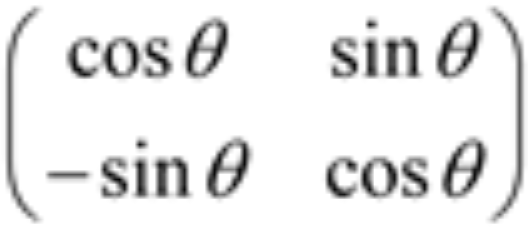
\includegraphics[scale=0.15]{trans}
 \end{figure}
 
 Hint: Remember that the imaginary number $i=\sqrt{-1}$ can be thought of a rotation of 90 degrees! (conventionally clockways).
  \subsection{Problem 2}
Using the equation
\begin{equation}
    V_i=\frac{1}{2}\epsilon_{ijk}T_{jk}
\end{equation}show that if $T_{jk}$ is a polar vector then $V_i$ is a pseudovector. What if $T_{jk}$ is a pseudovector?

Hint: Differentiate the expression and use the relationships $T'_{jk}=a_{j\alpha}a_{k\beta}a_{\alpha \beta}$ and $\epsilon'_{ijk}=det(A)a_{im}a_{jn}a_{kp}\epsilon_{mnp}$
  \subsection{Problem 3}
For Cartesian (rectangular) coordinates, the linear element is expressed as $ds^2=dx^2+dy^2+dz^2$. Find the line element $ds^2$ for cylindrical coordinates.

Hint: draw a circle of radius $r$ in the $x-y$ plane to derive a relationship between rectangular and cylindrical coordinates.
\subsection{Problem 4}
Find the linear element $ds^2$, the vector $d\bm{s}$, the volume element $dV$ and the base vectors $\bm{a}$ and $\bm{e}$ for parabolic cylinder coordinates $(u,v,z)$, where:
\begin{equation}
    x=\frac{1}{2}(u^2+v^2)
\end{equation}
\begin{equation}
    y=uv
\end{equation}
\begin{equation}
    z=z
\end{equation}
\begin{figure}[h]
    \centering
    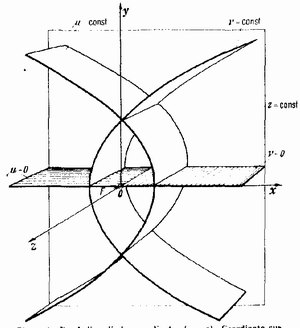
\includegraphics[scale=0.75]{4}
    \caption{Parabolic cylinder coordinates}
    \label{fig:my_label}
\end{figure}
  
\end{document}
